\newpage
\section{Generalised Negative Binomial Distribution}
\subsection*{Introduction}
The \emph{negative binomial} distribution, NB, was first proposed almost 
100 years ago in 1920 by Greenwood \& Woods, \cite{greenwood1920inquiry}, 
but its generalisation for both \emph{binomial} and NB distributions called the 
\emph{generalised negative binomial distribution}, GNB, was found 
more then 50 years later by Jain \& Consul (1971), \cite{jain1971generalized}. 
The PMF of the GNB is defined for $0<\alpha<1$ and $|\alpha \beta| < 1$ 
and reads in Jain \& Consul paper
\begin{align*}
b_{\beta}(x,n,\alpha) &= 
\frac{n \; \Gamma(n+\beta x)}{x! \;\Gamma(n + \beta x - x +1)}  \; \alpha^x (1-\alpha)^{n+\beta x-x}, n>0, x=0,1,2,3,...
\end{align*}
such that $b_{\beta}(x,n,\alpha) = 0 \text{ for } x \leq m \text{ if } n+\beta m < 0.$\\
Interestingly, following distributions are special cases of the GNB distribution
\begin{itemize}
\item 
binomial, B(n,p)
\item 
negative binomial, NB(r,p)\footnote{This corresponds to the NB1 parameterisation 
of the negative binomial distribution in ProbOnto, \cite{Swat:2015a}.}
\item 
inverse binomial, IB(k,p)
\end{itemize}
which will be shown in the following sections. 

\begin{figure}[ht!]
\centering
  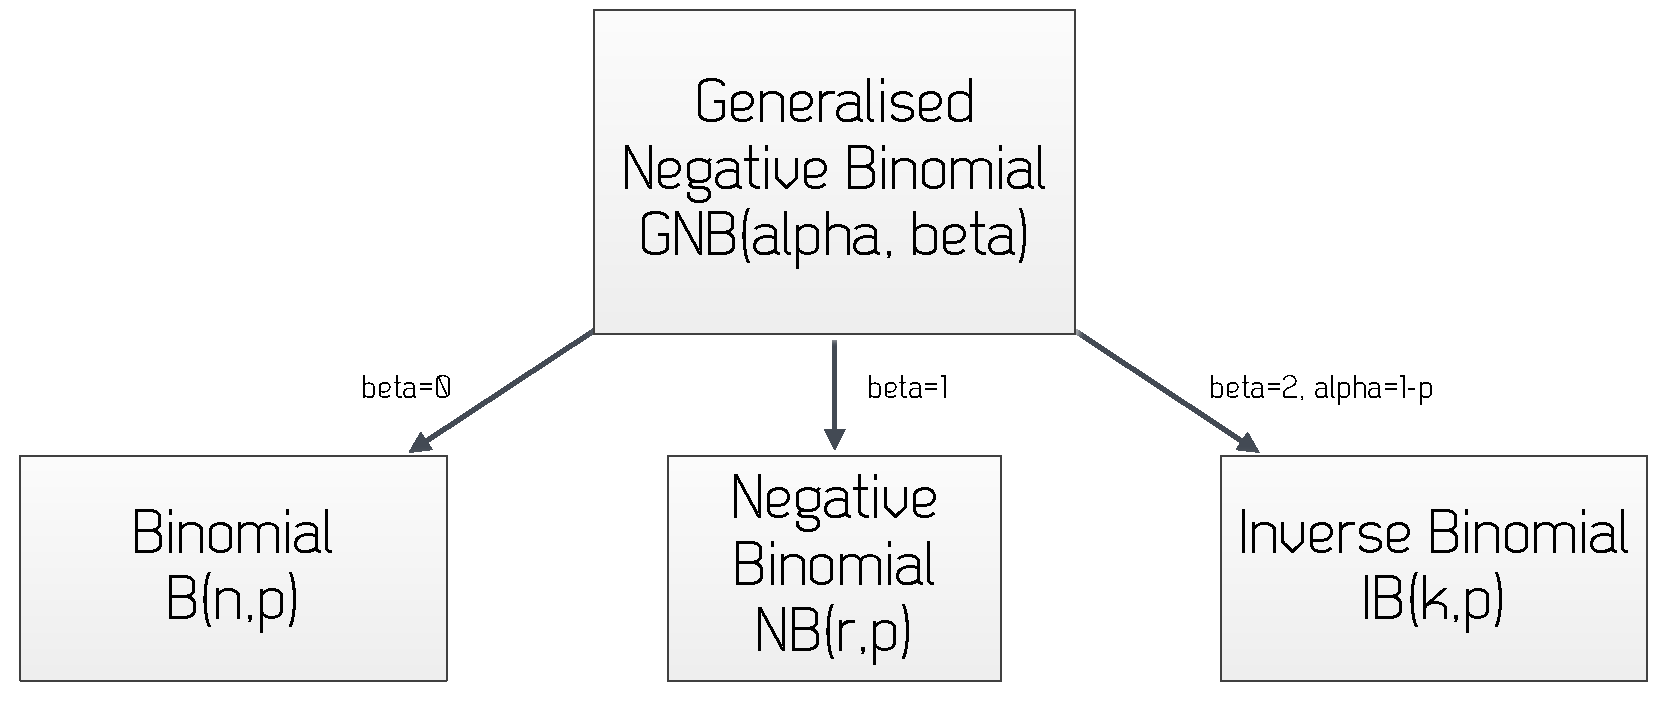
\includegraphics[width=120mm]{pics/GNBspecialCases.pdf}
 \caption{GNB and its family, see also \cite{Consul:2006qf}.}
 \label{fig:GNBspecialCases}
\end{figure}


\subsection*{GNB($\alpha$,$\beta$) $\rightarrow$ B($n$,$p$)}
According to Jain \& Consul, \cite{jain1971generalized}, GNB reduces to B for $\beta = 0$ and 
indeed this can be shown (replacing $\alpha$ with $p$) as follows
\begin{align*}
 b_{\beta}(x,n,\alpha) \rightarrow P_{B}(x;n,p): %= \binom {k+r-1}k (1-p)^r p^k \nonumber
 \frac{n \; \Gamma(n+\beta x)}{x! \;\Gamma(n + \beta x - x +1)}  \; \alpha^x (1-\alpha)^{n+\beta x-x} \rightarrow 
\frac{n \; \Gamma(n)}{x! \;\Gamma(n - x +1)}  \; p^x (1-p	)^{n-x} 
\end{align*}
with the first term in the last expression $\frac{n \; \Gamma(n)}{x! \;\Gamma(n - x +1)} = \frac{n (n-1)!}{x! (n-x)!} 
= \frac{n!}{x!(n-x)!} = {n \choose x}$ we get the expected result
\begin{align*}
P_{B}(x;n,p) = {n \choose x} p^x (1-p)^{n-x}. % \quad \text{ with } \quad 0<p<1, n>0, x=0,1,2,3,....
\end{align*}

\subsection*{GNB($\alpha$,$\beta$) $\rightarrow$ NB($r$,$p$)}
According also to Jain \& Consul, \cite{jain1971generalized}, GNB reduces to NB for $\beta = 1$ and 
indeed this can be shown (replacing $\alpha$ with $p$ and $n$ with $r$) as follows
\begin{align*}
 b_{\beta}(x,n,\alpha) \rightarrow P_{N\!B}(x;r,p):
 \frac{n \; \Gamma(n+\beta x)}{x! \;\Gamma(n + \beta x - x +1)}  \; \alpha^x (1-\alpha)^{n+\beta x-x} \rightarrow 
\frac{r \; \Gamma(r + x)}{x! \;\Gamma(r + 1)}  \; p^x (1-p)^{r} 
\end{align*}
with the first term $\frac{r \; \Gamma(r + x)}{x! \;\Gamma(r + 1)} = \frac{r \; (r + x - 1)!}{x! \;r!} = \frac{(r + x - 1)!}{x! \;(r-1)!}
= {r + x - 1 \choose x}$ we get the correct PMF
\begin{align*}
P_{N\!B}(x;r,p) = {r + x - 1 \choose x} p^x (1-p)^r  .
\end{align*}


\subsection*{GNB($\alpha$,$\beta$) $\rightarrow$ IB($k$,$p$)}
Yanagimoto, \cite{yanagimoto1989inverse}, proposed the \emph{inverse binomial} 
distribution as another special case of GNB for $\beta = 2, \alpha=1-p$ and $n=k$, which 
can be derived as the following shows 
\begin{align*}
b_{\beta}(x,n,\alpha) \rightarrow P_{I\!B}(x;k,p):
 \frac{n \; \Gamma(n+\beta x)}{x! \;\Gamma(n + \beta x - x +1)}  \; \alpha^x (1-\alpha)^{n+\beta x-x} \rightarrow 
\frac{k \; \Gamma(k + 2x)}{x! \;\Gamma(k + x + 1)}  \; (1-p)^x p^{k+x} 
\end{align*}
and the result follows in agreement with the formulation in \cite{yanagimoto1989inverse}, i.e.
\begin{align*}
P_{I\!B}(x;k,p) = \frac{k \; \Gamma(2x + k)}{\Gamma(x+1) \;\Gamma(x + k + 1)}  \; p^{k+x} (1-p)^x ,
\end{align*}
and from $|\alpha \beta| < 1$ and $0<\alpha<1$ one can derive the required condition for p, $1/2 < p < 1$.\\
Interestingly, IB has a medical application. Yanagimoto, \cite{yanagimoto1989inverse}, 
used the distribution it estimate the proportion of discharged patients who can be 
expected to stay completely free from some disease. In the original paper a dataset
for relapse of pulmonary tuberculosis was analysed.



\section*{Bios}
Here short bios of the people behind these distributions:

\begin{itemize}
\item 
Greenwood and Yule (1920), 'An inquiry into the nature of frequency 
distributions representative of multiple happenings with particular 
reference to the occurrence of multiple attacks of disease or of 
repeated accidents':
\begin{itemize}
\item 
Major Greenwood FRS (9 August 1880 - 5 October 1949) was 
an English epidemiologist and statistician born in Shoreditch in 
London's East End. He was elected President of the Royal Statistical 
Society in 1934 and awarded its Guy Medal in Gold in 1945.
\item 
Udny Yule FRS (18 February 1871 - 26 June 1951) was a 
Scottish statistician, born in Morham, near Haddington. He was active 
in the Royal Statistical Society, was also awarded its Guy Medal in Gold 
in 1911, and served as its president in 1924-26.
\end{itemize}
\item 
Jain and Consul (1971), 'A generalized negative binomial distribution':
\begin{itemize}
\item 
about Jain nothing is known on the web.
\item 
Prem C. Consul is professor emeritus at the Department 
of Mathematics and Statistics, University of Calgary, and author of 
books on Generalised Poisson and Lagrangian distributions 
\url{http://math.ucalgary.ca/math_unitis/profiles/prem-c-consul}
\end{itemize}
\item 
Yanagimoto (1989), 'The inverse binomial distribution as a statistical 
model':
\begin{itemize}
\item 
Takemi Yanagimoto - professor at the Institute of 
Statistical Mathematics in Tokyo.
\url{http://www.ism.ac.jp/~yanagmt/eng.html}
\end{itemize}
\end{itemize}

















